\begin{problem}{小 H 的重启}{standard input}{standard output}{5 seconds}{256 megabytes}

某日,HZNU 的 OnlineJudge 服务器无法登录,导致 Hsueh- 不能在服务器上传题目。

经过艰苦的判断,Hsueh- 猜测这是因为服务器死机了。

可怜的 Hsueh- 就只能去机房重启服务器。

经过很长一段时间,Hsueh- 终于找到了机房,发现了服务器放的位置,可是他从来都没见过这台来自泛银河宇宙无敌无限公司超级非量子低速土豆服务器,一时间不知道该怎么重启。

回想起以前购买这台服务器时,有师傅上门安装,就没有关机过一次。

这让他束手无策。他只能给师傅打电话,可是师傅也忘了怎么操作。

最后师傅告诉他,说明书扔在了仓库的某个位置,并告诉了他坐标。这下 Hsueh- 终于能找到重启服务器的方法了!

当 Hsueh- 走进仓库却发现,由于之前的胡乱堆放,整个仓库非常混乱,即使知道坐标也需要翻越一些箱子。

因为箱子都是胡乱摆放的,因此它们不会重叠。

比如,仓库可能像下图一样。可以认为仓库无限大,而 Hsueh- 无限小,可视作一个点。

\begin{center}
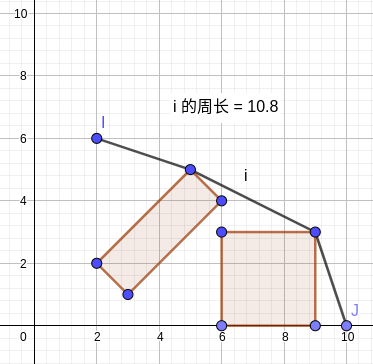
\includegraphics[width=8cm,height=10cm,natwidth=320,natheight=360]{data1.png} % 插入图片
\end{center}


由于箱子整天被搬来搬去,加上走了大量的路,最后实在不想翻越,因此他决定绕过箱子。同时,他希望走的路径最短。

不过,他想让你告诉他最短路径长度,方便他决定到底是重启服务器还是重新换一台泛银河宇宙无敌无限公司超级高级不可说神仙服务器。



\InputFile
第 $1$ 行 $1$ 个数字 $n$($0 \leqslant n \leqslant 200$),表示仓库中的箱子个数。

接下来 $n$ 行,每行 $8$ 个整数,$x_{i_0},y_{i_0},x_{i_1},y_{i_1},x_{i_2},y_{i_2},x_{i_3},y_{i_3}$,按照逆时针方向排列,表示一个矩形箱子。

第 $n+2$ 行,$4$ 个整数,$x_0,y_0,x_1,y_1$,分别表示 Hsueh- 的坐标和说明书的坐标。

所有整数的绝对值均不超过 $10000$。

输入保证不会出现两个箱子的顶点重合,同时保证一个箱子的顶点不会出现在另一个箱子的边上面。

\OutputFile
输出一行,为一个浮点数,假设你的答案为 $a$,标程的答案为 $b$,你的答案被认为是正确的当且仅当满足 $\frac{|a - b|}{\max{(1, |b|)}} \le 10^{-4}$。


\Example

\begin{example}
\exmpfile{example.01}{example.01.a}%
\end{example}

\end{problem}

